\section{Problem Statement}
\label{sec:statement}

% \begin{center}
% \begin{tikzpicture}[scale=1.75, every node/.style={scale=0.75}]
%   \clip (-1.1,-0.5) rectangle (4.8,4.2);
%   \draw[thin] (0,0) rectangle (4,3);
%   \draw (0,0) -- (4,3);
%   \draw (1.0, 2.0) circle [radius=1cm];
%   \draw (3.0, 1.0) circle [radius=1cm];
%   \draw (1.0, 2.0) -- (3.0, 1.0);
%   \filldraw (1.0, 2.0) circle [radius=0.2mm];
%   \filldraw (3.0, 1.0) circle [radius=0.2mm];
%   \draw (1.0,2.0) node[above left] {$X$};
%   \draw (3.0,1.0) node[below] {$Y$};
%   \draw (2.0,0.0) node[below] {$w$};
%   \draw (4.0,1.5) node[right] {$h$};
% \end{tikzpicture}
% \end{center}

The original problem is stated as in the caption of Figure~\ref{fig:problem}.
However, we will extend the statement slightly to make it a tiny bit more
interesting.  Let $r$ be the radius of the circles and pose the following
questions:

\begin{figure}[h]
  \centering
  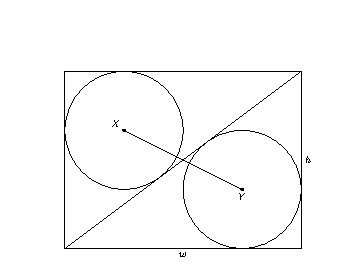
\includegraphics[trim={0 0 0 1.2cm},clip,width=0.5\textwidth]{./figures/basic1.pdf}
  \vspace{-8mm}
  \caption{Given the width $w$ and height $h$ of the rectangle, find the length
  of the line segment $XY$ between the centres of the inscribed circles, which
  have the two adjacent sides of the rectangle and its diagonal as tangents.}
  \label{fig:problem}
\end{figure}

\begin{enumerate}
  \setlength\itemsep{0em}
  \item Find the map $f: \mathbb{R}_+^2 \rightarrow \mathbb{R}_+^2$ that takes
          the side lengths of the rectangle $(w,h)$ to $(r, \abs{XY})$, the
          radius of one of the circles and the length of the line segment $XY$.
  \item Find the inverse $f^{-1}$ of $f$, that takes $(r, \abs{XY})$ to $(w,h)$.
\end{enumerate}

